\section{Electric Motor background}
In current days, a lot of effort and research are focusing in electric motor design: it is one of the key component for the electrification process of the automotive industries.

There are many types of motors that can be used in automotive applications, and one of the most common is the \gls{pmsm}: as the name says, it is a synchronous motor using magnets to create the magnetic field that moves the rotor. An example of a disassembled \gls{pmsm} in \cref{fig:PMSM_figure}.
\begin{figure}[H]
    \centering
    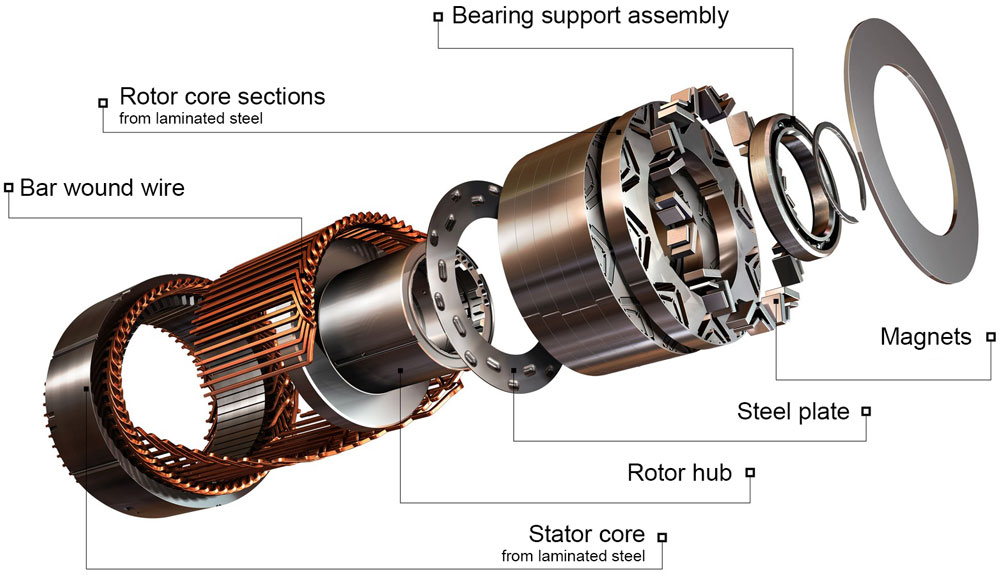
\includegraphics[width=0.7\textwidth]{sections/images/section1/ipmsm_disassembled_w1000.jpg}
    \caption{Working Components of \gls{pmsm}\cite{pmsm_review}}
    \label{fig:PMSM_figure}
\end{figure}
\subsection{Type of motor chosen}
There are different ways to design a \gls{pmsm}\cite{pmsm_review}, that won't be covered in this paper. For the sake of simplicity, in this project it has been decided to focus on a specific design configuration of electric motor, otherwise the dataset creation would become too complex, and much more experience would be needed in \gls{pmsm} design.

The two main part of an electric motor are the \emph{Stator} and the \emph{Rotor}, for both there are different design that could be chosen.

\textbf{DISCLAIMER}: Here i am assuming to use simplified notation, that could differ to precise keywords used in literature. This section is not a design review of electric motors, but just an help understanding some key design concept
\subsubsection{Rotor design chosen}
As it is the most simple \gls{pmsm} type to study and to deal with, \gls{spm} rotor has been chosen to create the dataset. The second motivation to this choice is that this design has been already covered by a previous university course here at MUNER\cite{MUNER}.

The characteristic of an \gls{spm} rotor is to have the magnets round shaped, and placed in the outer side of the rotor (as can be seen in \cref{fig:rotor_magnet_placement})

\begin{figure}[H]
    \centering
    \makebox[\textwidth][c]{
    %
    \begin{subfigure}{0.55\textwidth}
        \centering
        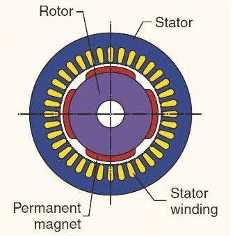
\includegraphics[width=.7\linewidth]{sections/images/section1/spm_example.jpg}
        \label{fig:spm_example}
        \caption{\glsxtrlong{spm}}
    \end{subfigure}
    %
    \begin{subfigure}{0.55\textwidth}
        \centering
        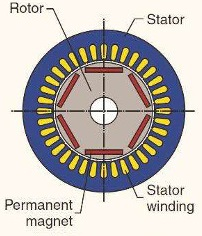
\includegraphics[width=.68\linewidth]{sections/images/section1/ipm_example.jpg}
        \caption{Interior Permanent Magnet}
        \label{fig:ipm_example}
    \end{subfigure}}
  \caption{Two of the most used rotor magnet placement}
  \label{fig:rotor_magnet_placement}
\end{figure}

\subsubsection{Winding layout chosen}
The decision of the stator design was easier due to the fewer option available.

The two main stator design (or better, winding layout) are \gls{dw} and \gls{fw}. There are advantages and disadvantages for both layouts, but \gls{fw} has been preferred for this project because demagnetization is more difficult to predict analytically. An example in \cref{fig:winding_placement}
\begin{figure}[H]
    \centering
    \makebox[\textwidth][c]{
    %
    \begin{subfigure}{0.55\textwidth}
        \centering
        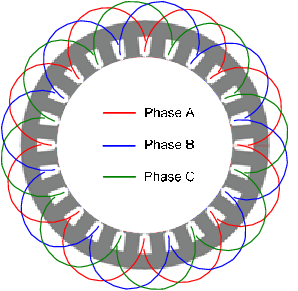
\includegraphics[width=.7\linewidth]{sections/images/section1/distribuited.png}
        \label{fig:dw_example}
        \caption{\glsxtrlong{dw}}
    \end{subfigure}
    %
    \begin{subfigure}{0.55\textwidth}
        \centering
        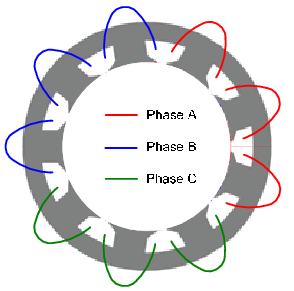
\includegraphics[width=.7\linewidth]{sections/images/section1/fractional.png}
        \caption{\glsxtrlong{fw}}
        \label{fig:fw_example}
    \end{subfigure}}
  \caption{Two of the most used rotor Winding layout}
  \label{fig:winding_placement}
\end{figure}

The wire inside the slots have been simplified as a normal round copper wire, without considering skin effects. Different copper inside slots can be seen in \cref{fig:copper_example}
\begin{figure}[H]
    \centering
    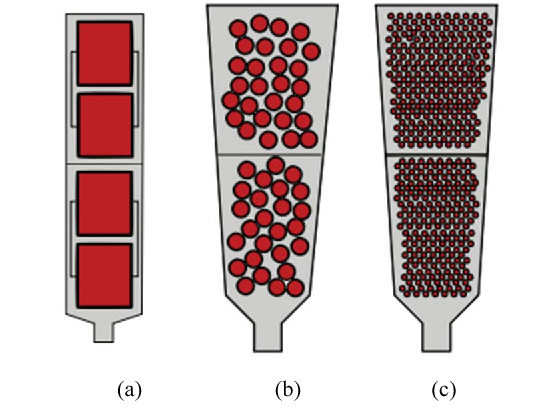
\includegraphics[width=0.5\textwidth]{sections/images/section1/copper_example.png}
    \caption{Slot area view: (a)hairpin, (b)round wire, (c)litz wire}
    \label{fig:copper_example}
\end{figure}
\subsection{Description of the problem}
Demagnetization of \gls{pmsm} motors is a tedious topic in high performance machines: It does happen due to high temperatures and high electric load during the utilization of the motor.

Demagnetization of a magnet happens if the magnetic field inside the magnet $H_{magn}$ is greater, in module, of its intrinsic coercivity $H_{CI}$(that depends on the material and the temperature of the magnet).

The analytical equation that describe when demagnetization happens is:
\begin{equation}\label{eq:demagn_formula_approx}
    |H_{magn}| = \left|\frac{\frac{N}{2}I-\frac{\delta_0}{\mu_0}B_r}{l_{magn}+\delta_0\frac{\mu_d}{\mu_0}}\right|<|H_{CI}|
\end{equation}
where
\begin{itemize}
    \item $N$: Series conductors per phase.
    \item $I$: Peak current crossing the windings.
    \item $\delta_0$: Airgap thickness.
    \item $\mu_0$: magnetic permeability of free space.
    \item $B_r=B_{r0}(1+\alpha_{B_{r}}(T-T_0))$: Magnet remanence.
    \item $l_{magn}$: magnet thickness.
    \item $\mu_d$: Permeability of the magnet.
    \item $H_{CI}=H_{CI0}(1+\alpha_{H_{CI}}(T-T_0))$: intrinsic coercivity
    \item $H_{CI0},B_{rI0}$: Reference Value.
    \item $\alpha_{H_{CI}}, \alpha_{B_{r}}$: temperature coefficient.
\end{itemize}

The downside of this equation, is that it assumes that the magnetic field produced by the magnet is sinusoidal, without taking in consideration side harmonics. 

\gls{fw} motors are known to produce an higher number of side harmonics, so this formula is not particularly suited for that stator type.

Another way to check demagnetization is to measure the $H_{magn}$ value inside magnets using \gls{fem} Software.

Temperature was set to the magnet temperature limit: $T=\SI{140}{\celsius}$ as datasheet. Magnet used is \emph{Cibas ren35h NeFeb}.
\subsection{Why this work could be useful?}
As already said, it is possible to check for demagnetization using using \gls{fem}, but that approach has different disadvantages:
\begin{itemize}
    \item The duration of \gls{fem} simulation can last up to tens of minutes $\rightarrow$ Design optimization time will be considerable.
    \item \gls{fem} simulation can only be used at the end ot the motor design process, when geometry has already been shaped $\rightarrow$ Precise prediction for demagnetization is not possible during early design stages.
\end{itemize}

This two disadvantages are particularly bad for high performance \gls{pmsm} motors used in automotive: those type of machines are usually pushed to the limit by exploiting their \gls{ol} capability.
\subsubsection{\texorpdfstring{\glsxtrlong{ol}}{Overload} of a motor}
The \gls{ol} is an important features of high performance electric motors: it is possible to inject more current, for a short interval of time time, and produce more torque than what the motor was built for.

How is it possible to run in \gls{ol} without damaging the motor? the electric/mechanic dynamics is relatively fast compared to the slow thermal dynamics: so to avoid overheating it is necessary to use \gls{ol} for a short period of time.

If the motor temperatures are kept in a safe range, the only concern about \gls{ol} is the demagnetization.
\subsubsection{\texorpdfstring{\glsxtrlong{ol}}{Overload} and Demagnetization}
As the approximated equation in \cref{eq:demagn_formula_approx} suggest, demagnetization can happen if the current $I$ is too high. This mean that for each motor it is possible to have a maximum overload current that it is not possible to exceed.
it can be useful to predict how much \gls{ol} it is possible to apply for two main reason:
\begin{itemize}
    \item Predict \gls{ol} at early development stage to modify it if different behavior are desired.
    \item Apply optimization algorithm at high speed.
\end{itemize}
\subsection{Proposed target of this work}
The target of this work is to create a machine learning tool capable to predict how much \gls{ol} is possible without going in demagnetization, given few initial parameters.

This work is made purely for didactic purpose, this is why a single type of motor is investigated, and limited parameters/materials can be chosen.

